\documentclass[10 pt,a4paper, openany]{article}
%titlepage
\usepackage[hidelinks]{hyperref}
\usepackage[italian]{babel}
\usepackage[T1]{fontenc}
\usepackage[utf8x]{inputenc}
\usepackage{amsfonts}
\usepackage{multicol}
\usepackage{graphicx}
\usepackage{amsmath}
\usepackage{framed}
\usepackage{extarrows}
\usepackage{cancel}
\usepackage{eurosym}
\usepackage{listingsutf8}
\usepackage{lastpage}
\usepackage{rotating} 
\usepackage{multirow}

\usepackage{caption}
\usepackage{makecell}
\usepackage{longtable}
\usepackage{array}
\usepackage{placeins}
\date{}


\usepackage{makeidx}
\makeindex
\usepackage{fancyhdr}
\pagestyle{fancy}
\lhead{
\includegraphics[width=.6cm]{../../../../../file_comuni/immagini/obelisk_sample_02.png}
  Obelix Group}
\chead{}
\rhead{\rightmark }% \leftmark}%da rimettere
\lfoot{}
\cfoot{}
\rfoot{\thepage / \pageref*{LastPage}}
%%%%%%%%%%%%%%%%%%%%%%%%%%%%%%%%%%%%%%
%\usepackage{lipsum}
\usepackage{../../../../../file_comuni/copertina2}
\nomedoc{Verbale esterno 2017-08-04}
\versione{v1\_0\_0}
\datacreazione{2017-08-04}
\verifica{Riccardo Saggese}
\approvazione{Nicolò Rigato}
\redazione{Emanuele Crespan \eanche Federica Schifano}
\uso{interno}
\distribuzione{Prof. Tullio Vardanega \eanche Prof. Riccardo Cardin \eanche Red Babel \eanche Gruppo Obelix}
\sommario{Verbale dell'incontro tra il gruppo \emph{Obelix} e il
  proponente \emph{RedBabel} in data 2017-08-04}


\begin{document}
\paginatitolo
\section{Informazioni sulla riunione}

\begin{itemize}
\item[] Data: 2017-08-04
\item[] Luogo: Residenza membro gruppo Obelix e sede Red Babel - videoconferenza
\item[] Ora: 11:00
\item[] Durata: 30'
\item[] Partecipanti interni: Obelix
  \begin{itemize}
  \item[] Emanuele Crespan
  \item[] Federica Schifano
  \item[] Nicolò Rigato
  \item[] Riccardo Saggese
  \item[] Silvio Meneguzzo
  \item[] Tomas Mali
  \end{itemize}
\item[] Partecipanti esterni: Red Babel
  \begin{itemize}
  \item[] Milo Ertola
  \item[] Alessandro Maccagnan
  \end{itemize}
\end{itemize}

\section{Argomenti trattati}

\begin{enumerate}
	\item Presentazione Interfaccia 
	\item Consigli e possibili cambiamenti
\end{enumerate}

	\clearpage


\section{Discussioni}
\begin{enumerate}
	\item Screenshot riguradanti l'apertura della SideArea laterale aggiunta su Rochet.chat e relative funzionalità sulle bolle da noi create.
	
		\begin{itemize}
			\item Schermata iniziale, dopo aver aperto la prima SideArea presente nella barra laterale destra
			
				\FloatBarrier
				\begin{figure}[ht]
					\centering
					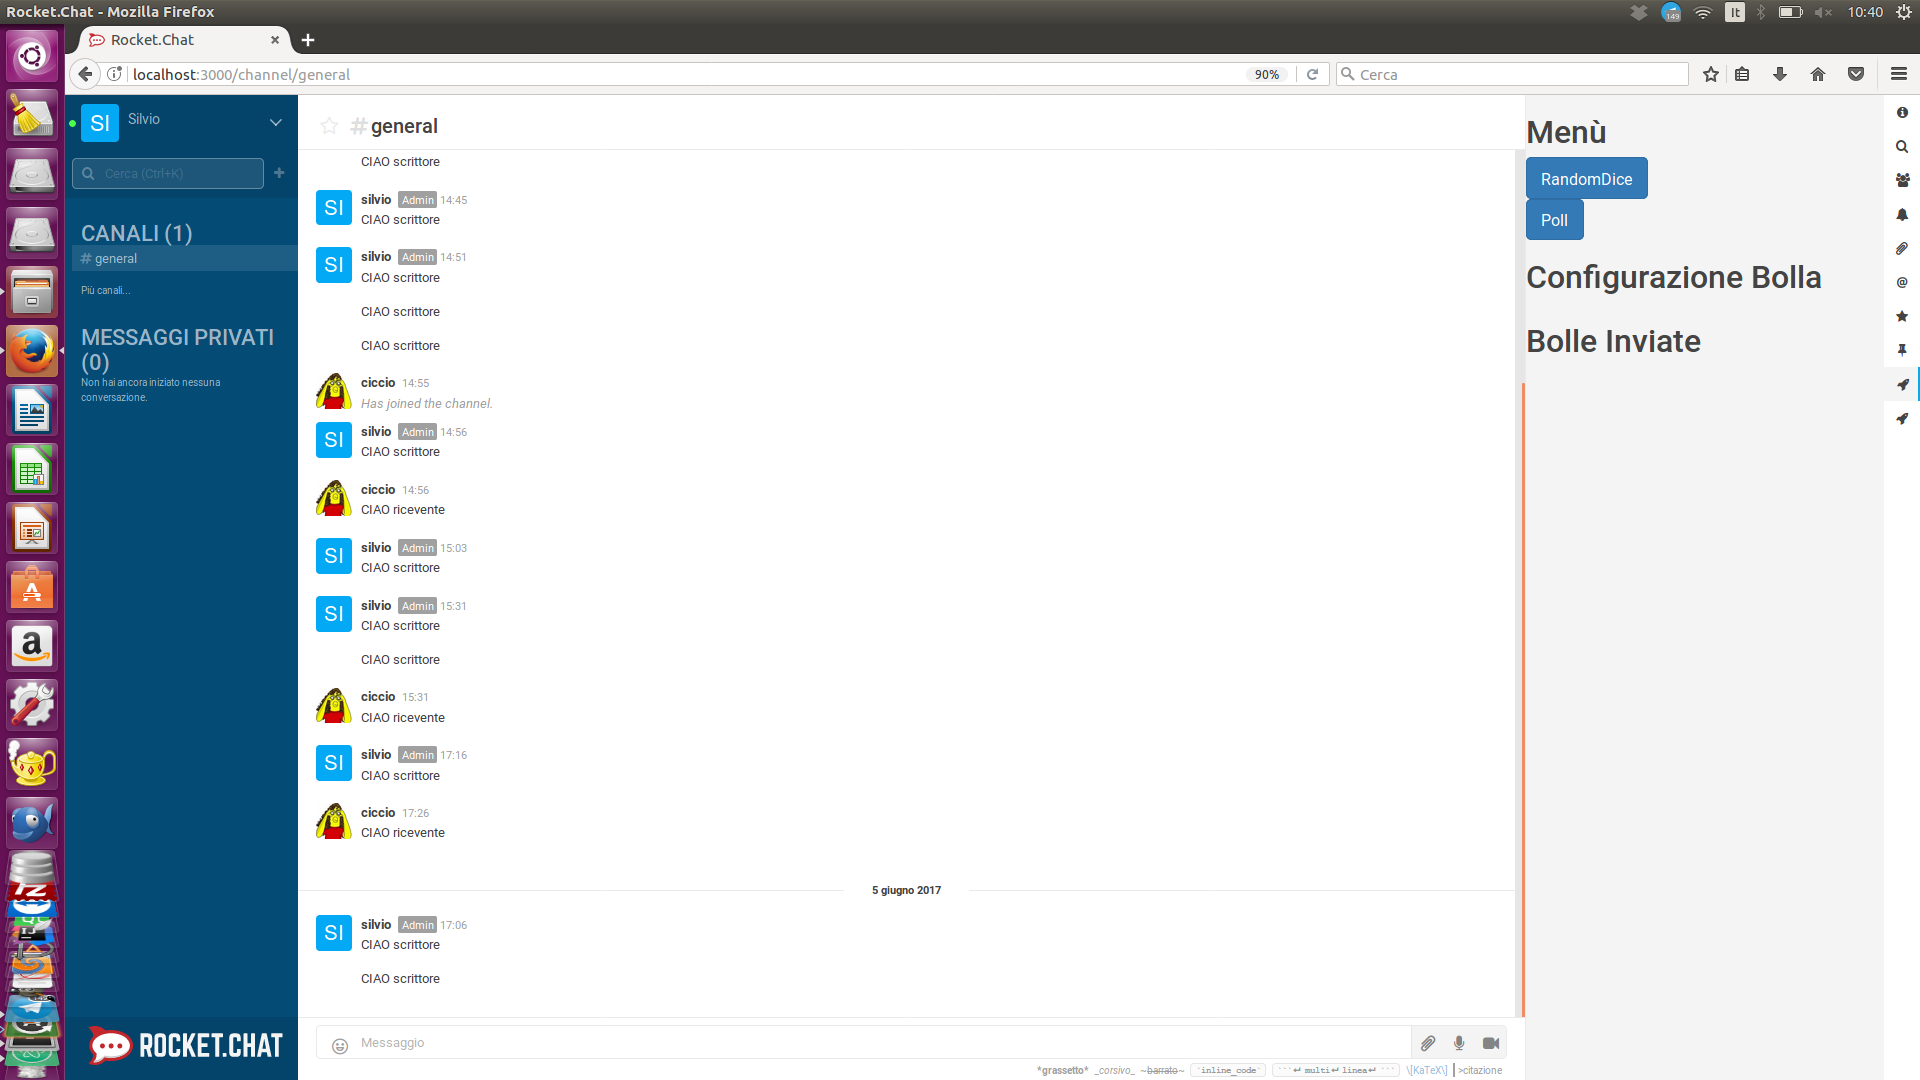
\includegraphics[scale=0.20]{img/1.png}
					\caption{aperta SideArea1}
				\end{figure}
			
			\clearpage
			
			\item  Pulsante della bolla RandomDice premuto, con conseguente apertura del Menù di configurazione della suddetta bolla
			
				\FloatBarrier
				\begin{figure}[ht]
					\centering
					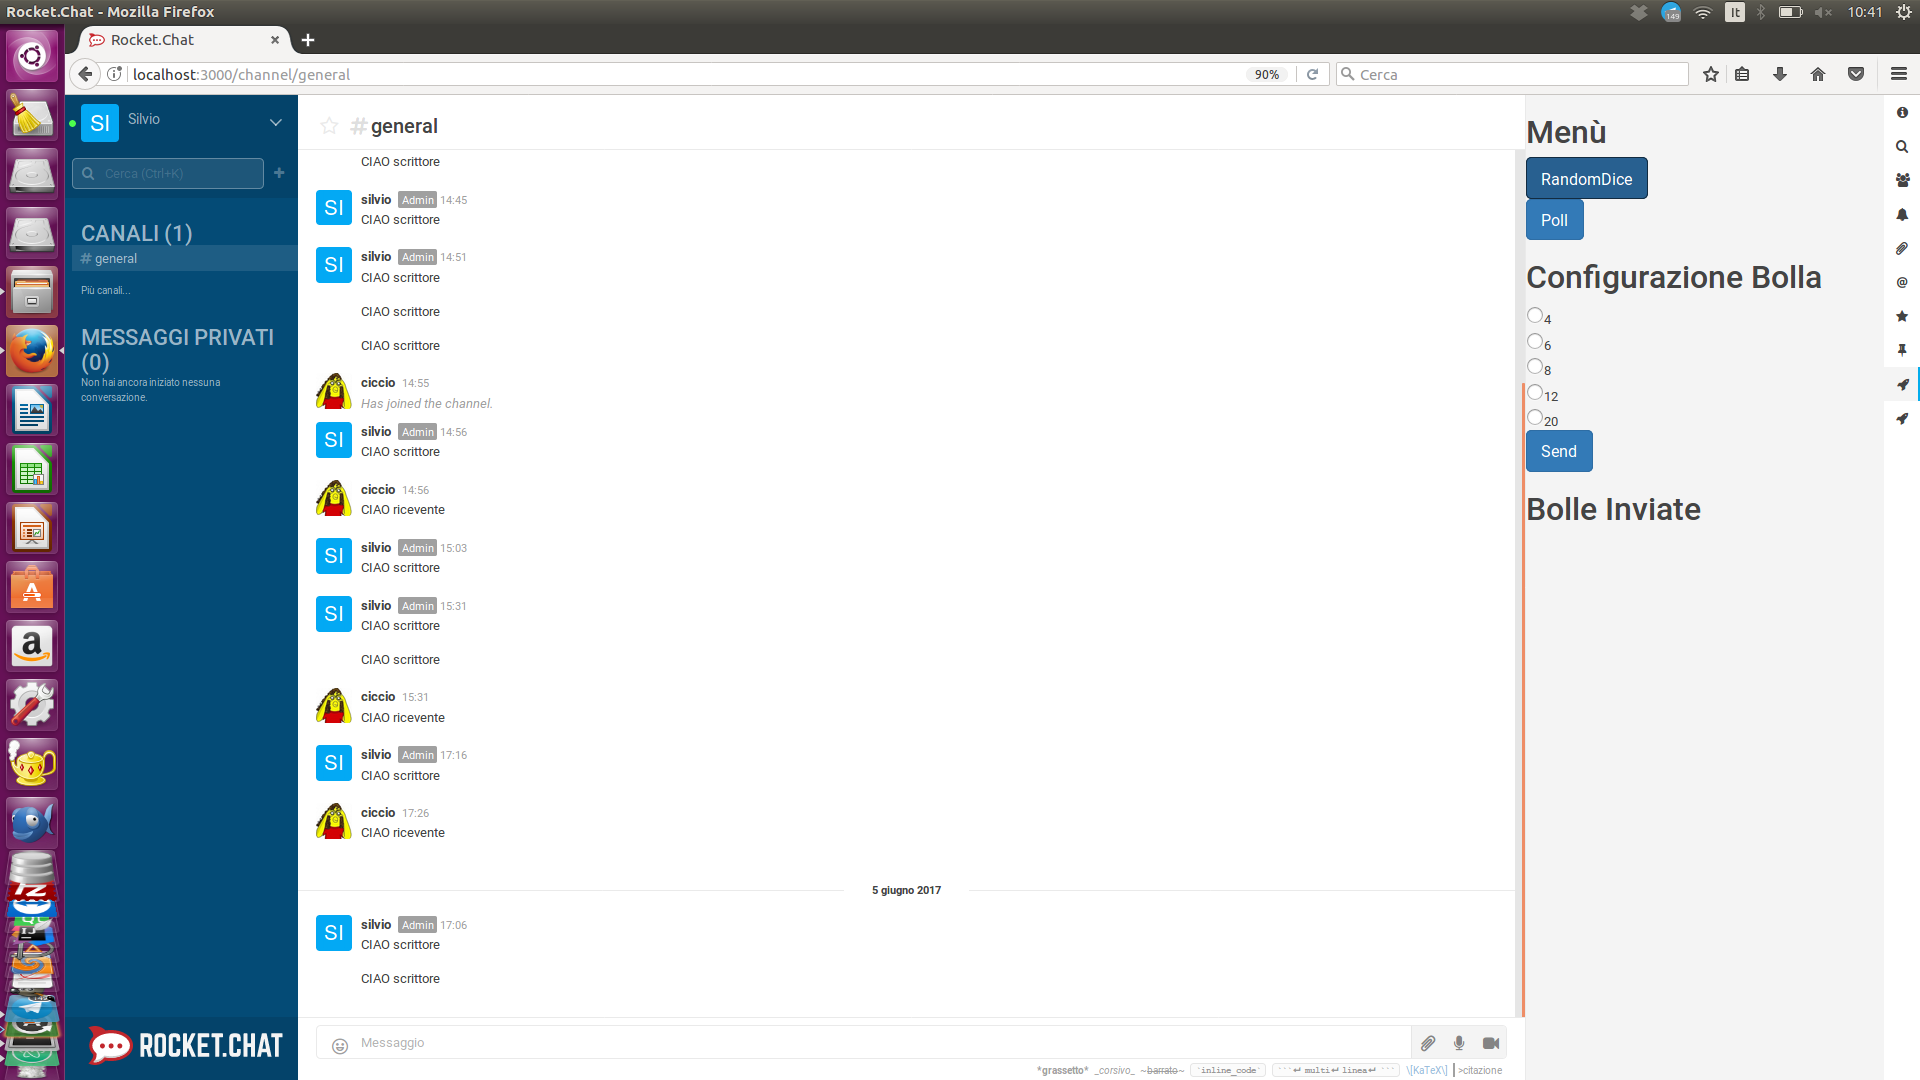
\includegraphics[scale=0.20]{img/2.png}
					\caption{premuto RandomDice}
				\end{figure}
			\clearpage
				
			\item Scelto il numero di facce del dado, con conseguente invio e attivazione della bolla random
			
				\FloatBarrier
				\begin{figure}[ht]
					\centering
					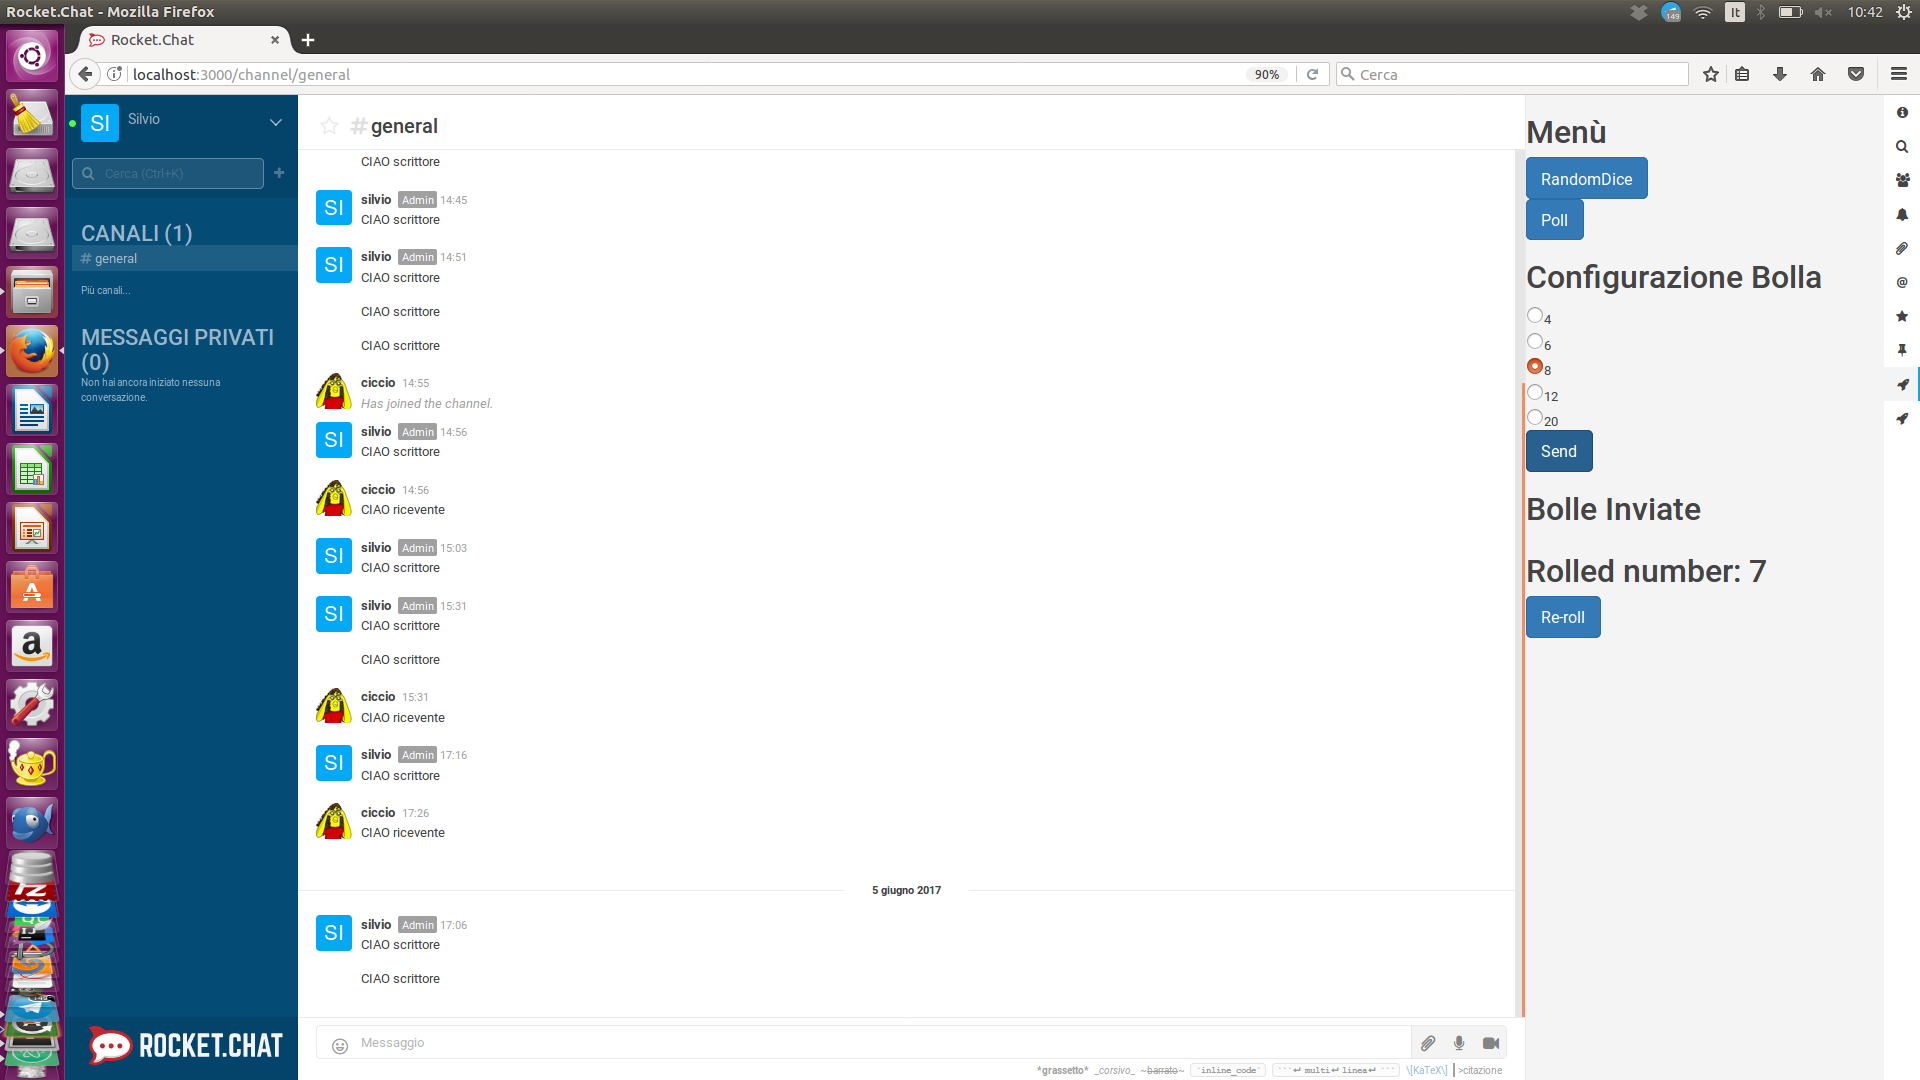
\includegraphics[scale=0.20]{img/3.png}
					\caption{RandomDice send}
				\end{figure}
				
			\clearpage
			
			\item Selezione bolla Poll nel Menù
			
				\FloatBarrier
				\begin{figure}[ht]
					\centering
					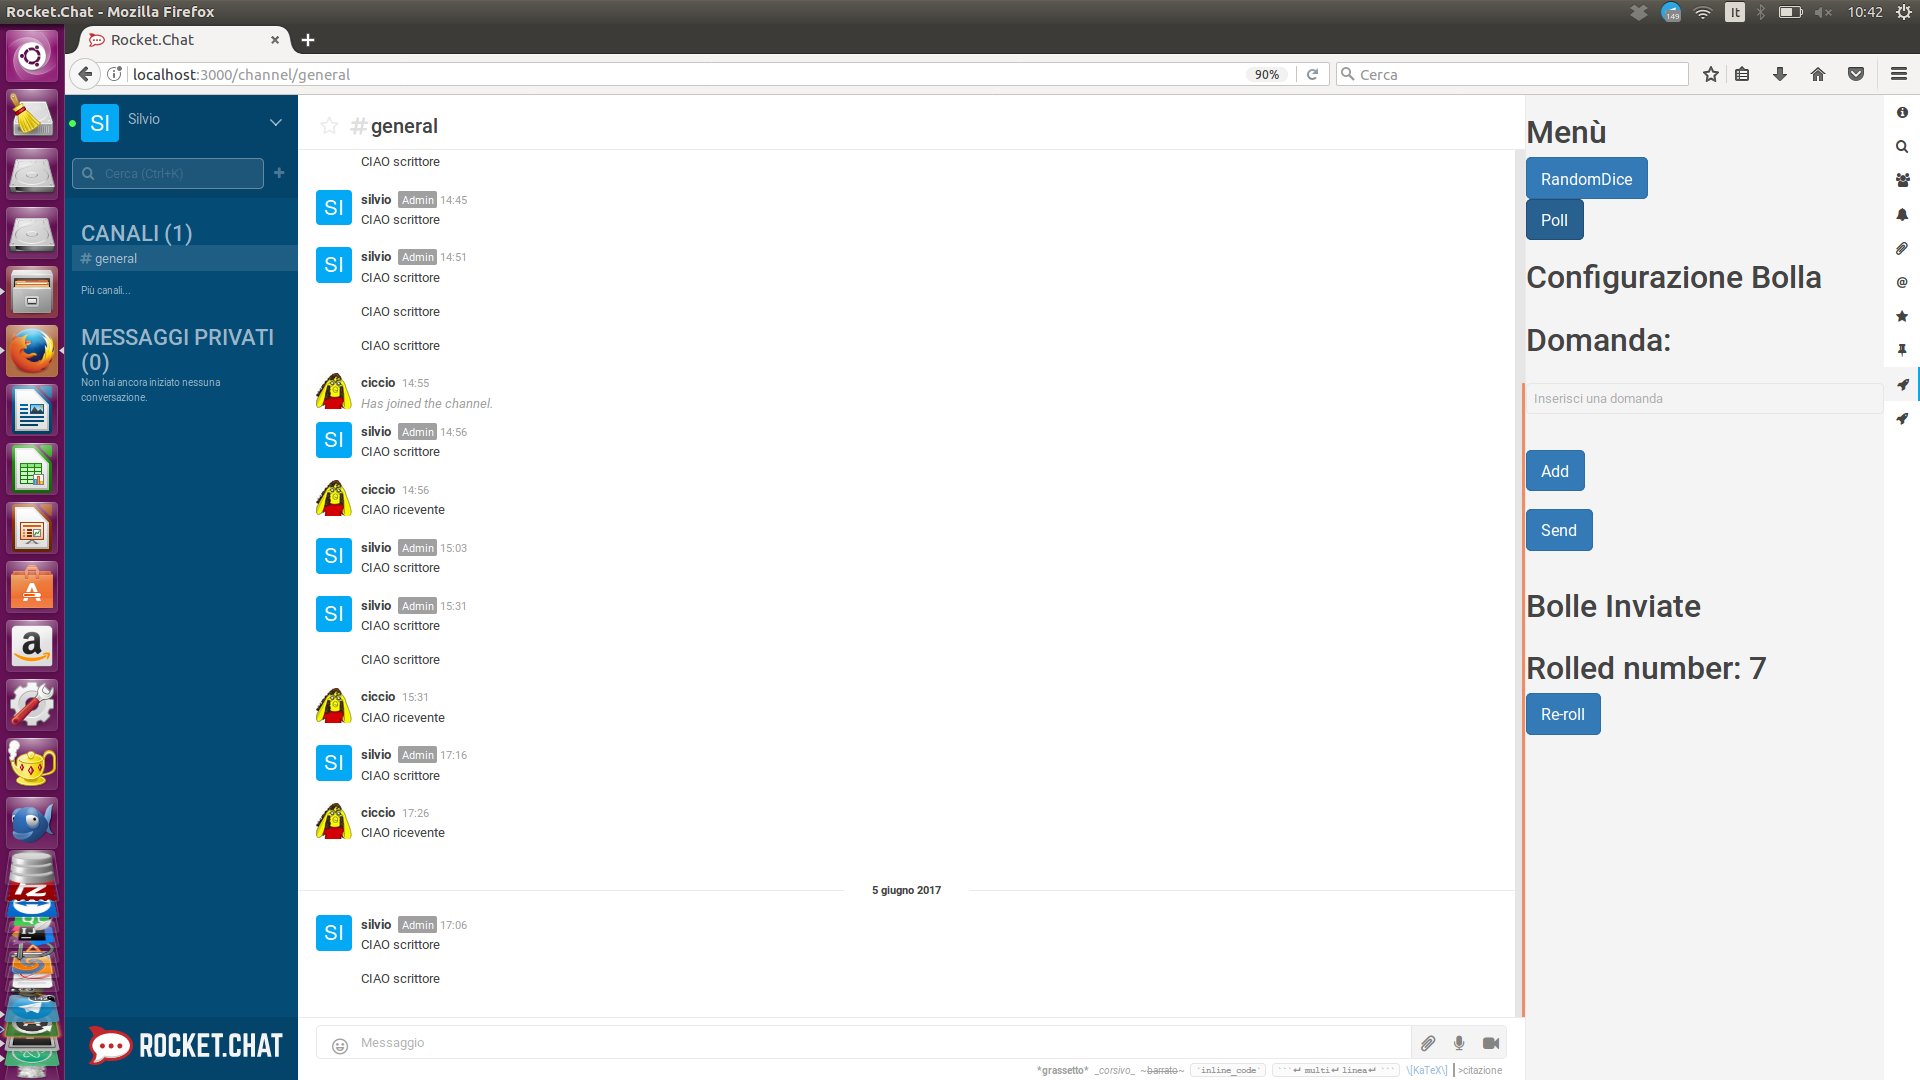
\includegraphics[scale=0.20]{img/4.png}
					\caption{premuto Poll}
				\end{figure}
			\clearpage
			
			\item Inserimento di una domanda e opzioni nella sezione di configurazione della bolla Poll
			
				\FloatBarrier
				\begin{figure}[ht]
					\centering
					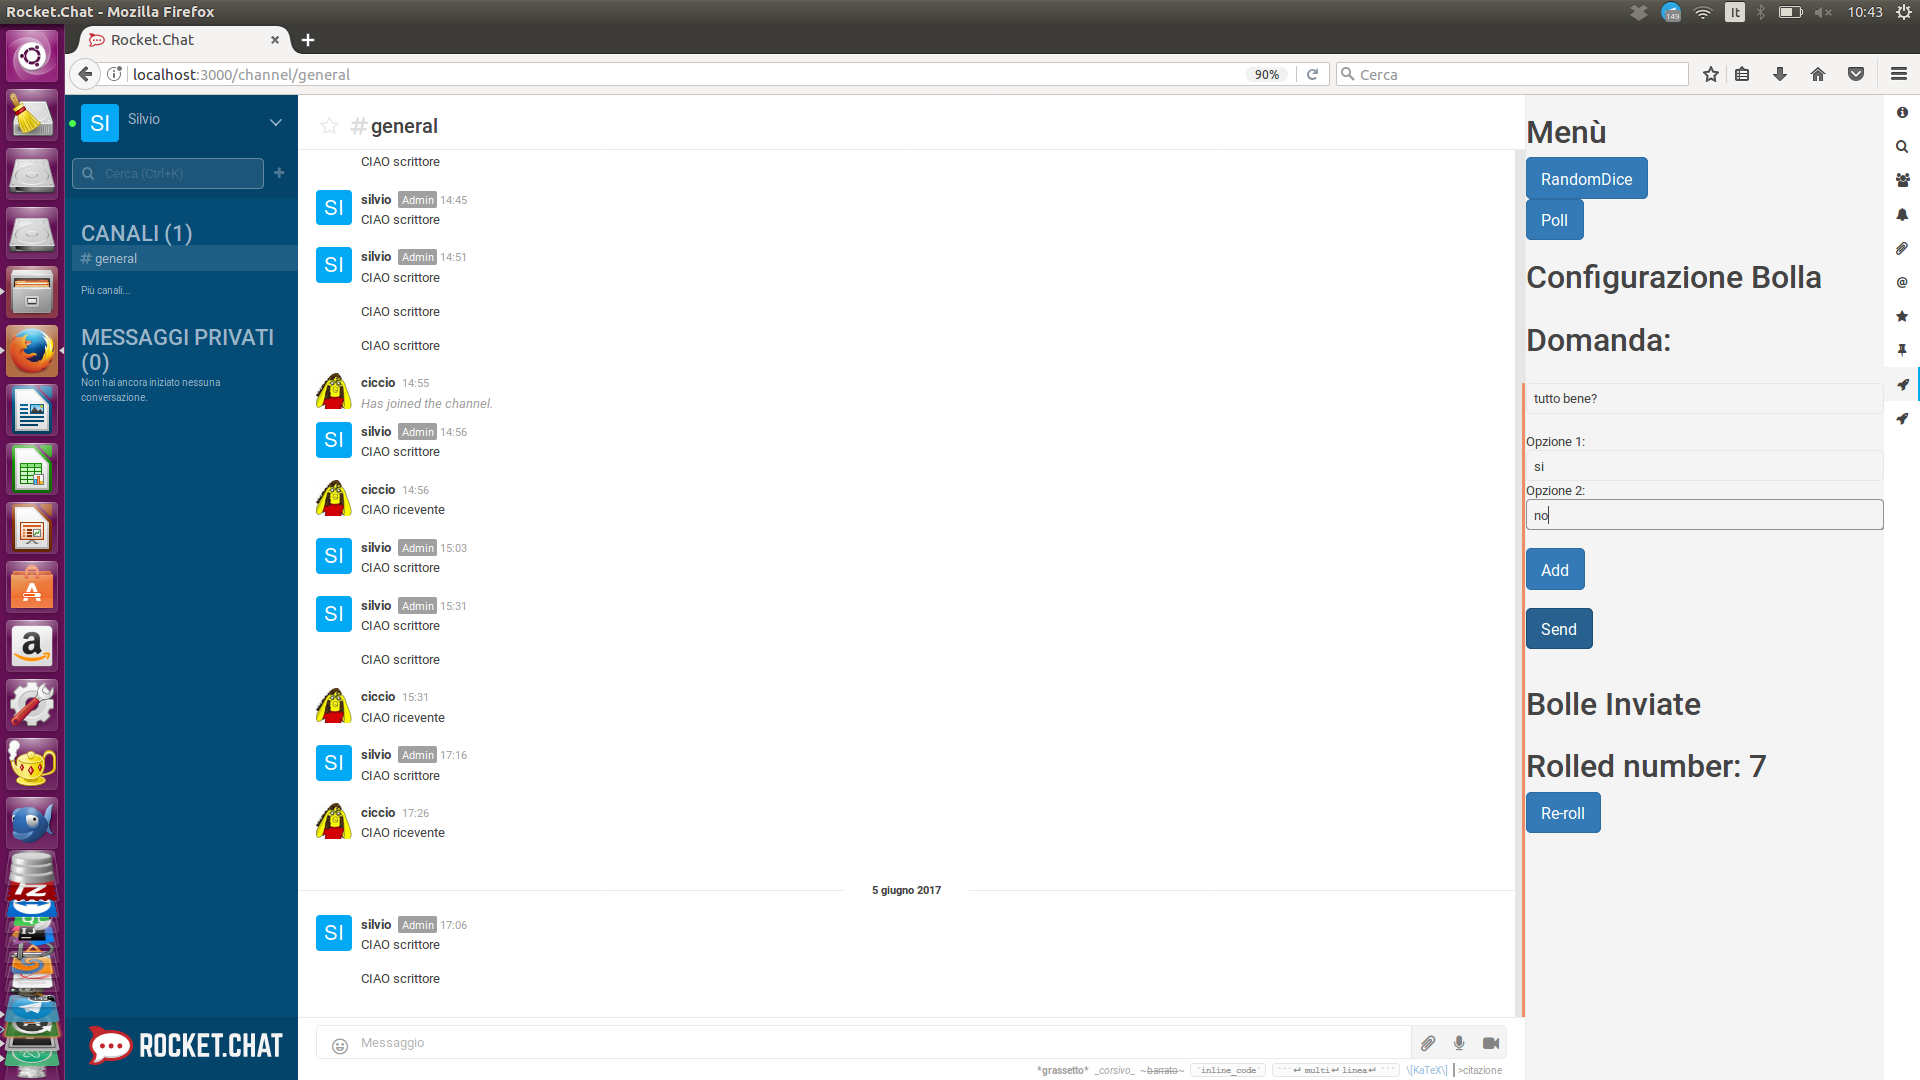
\includegraphics[scale=0.20]{img/5.png}
					\caption{configurazione Poll}
				\end{figure}
				\clearpage
				
			\item Send della bolla Poll e votazione
			
				\FloatBarrier
				\begin{figure}[ht]
					\centering
					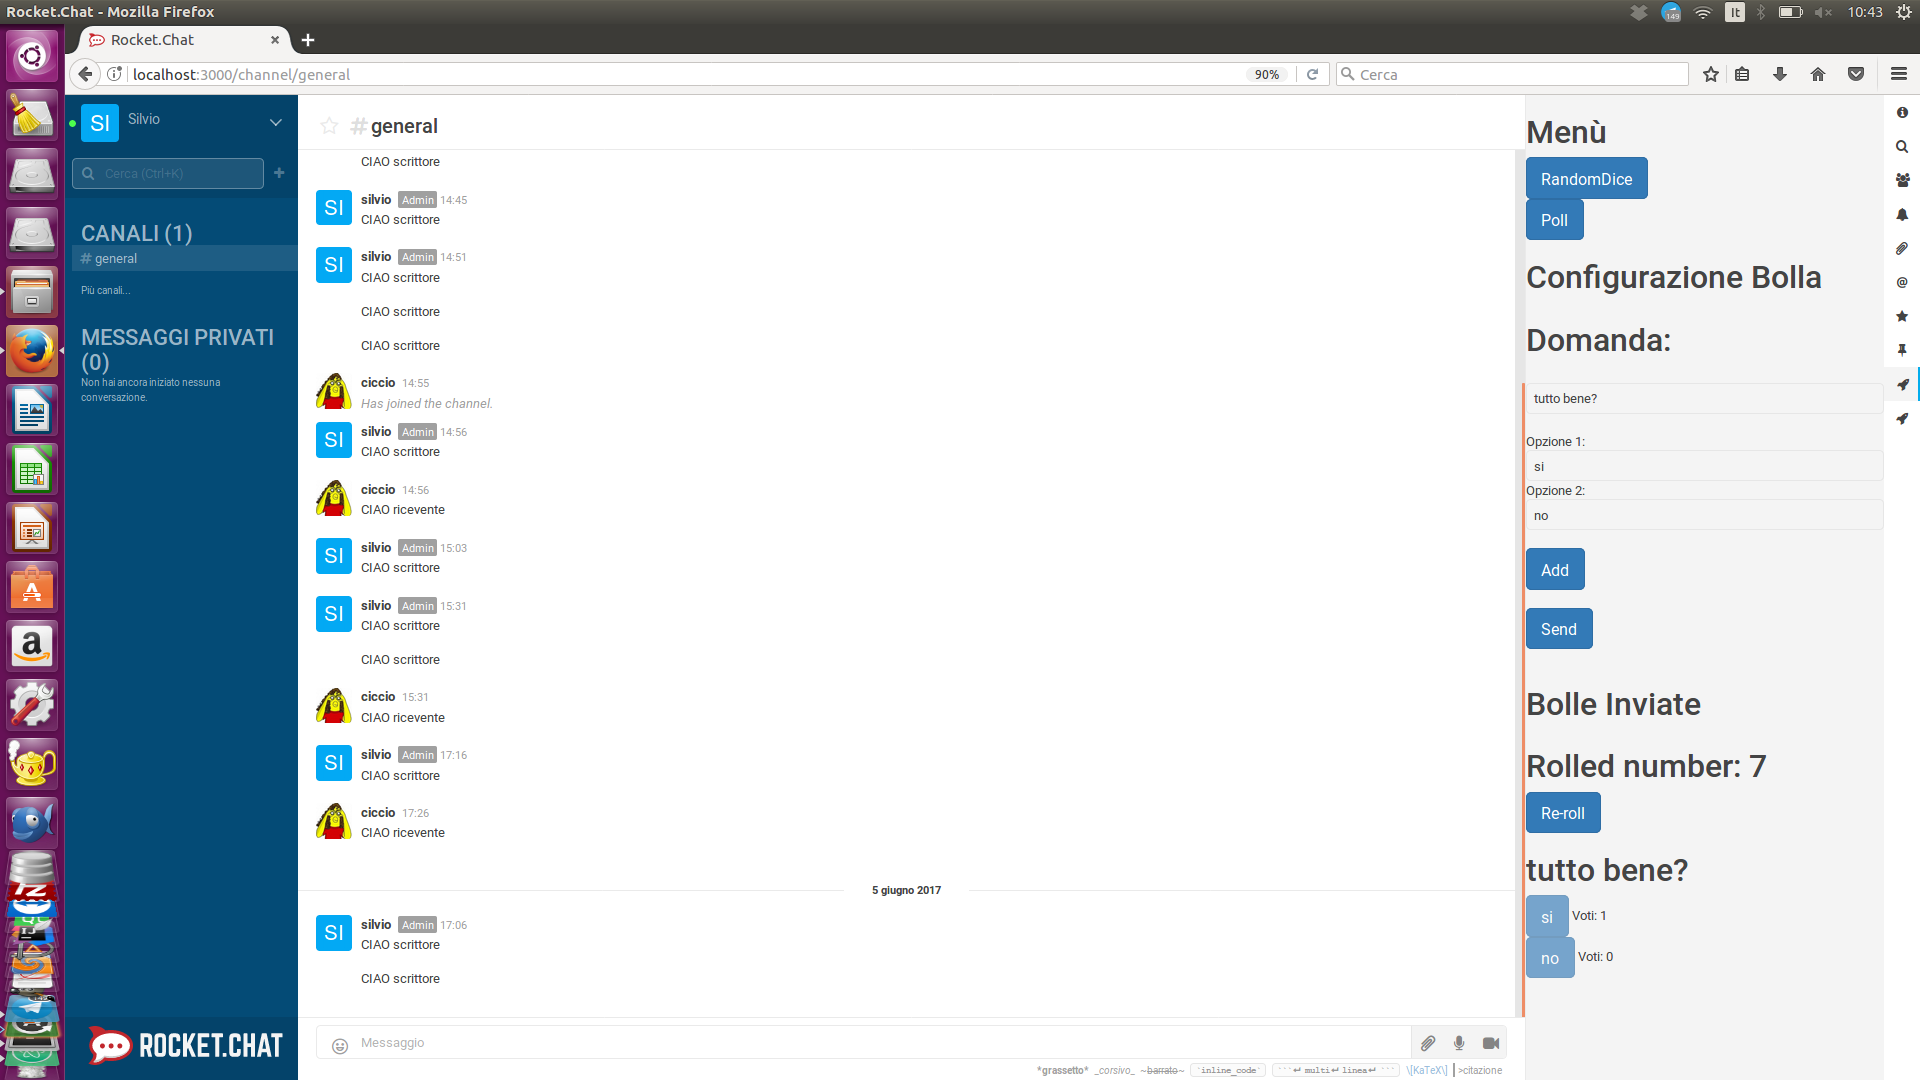
\includegraphics[scale=0.20]{img/6.png}
					\caption{Poll send}
				\end{figure}
			
		\end{itemize}


	Questa struttura è stata accettata come ottima idea da parte dei proponenti senza alcuna obiezione o possibile cambiamento
	

	
	
	\item Suggerimento: nell'uso di javascript attenersi ad un approccio meno simile alla programmazione ad oggetti.
	

	
\end{enumerate}



\end{document}
